\documentclass[tikz,border=3pt]{standalone}
\usetikzlibrary{positioning,arrows.meta,shapes.geometric,backgrounds}

\begin{document}
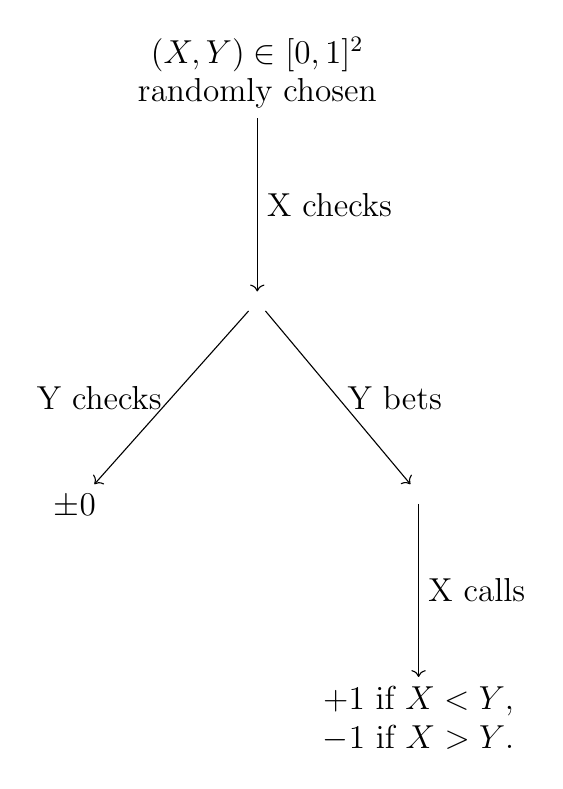
\begin{tikzpicture}

% nodes (manual positions for clearer layout)
\node[align=center, font=\large] (root) {$(X,Y)\in[0,1]^2$ \\randomly chosen};
\node[below=22mm of root] (xcheck) {};
\node[below left=22mm and 18mm of xcheck, font=\large] (ycheck) {$\pm 0$};
\node[below right=22mm and 18mm of xcheck] (ybets) {};
\node[align=center, below=22mm of ybets, font=\large] (xcall) {
$+1$ if $X < Y$, \\
$-1$ if $X > Y$.
};

% edges with labels
\draw[->] (root) -- (xcheck) node[midway,right, font=\large] {X checks};
\draw[->] (xcheck) -- (ycheck) node[midway,left, font=\large] {Y checks};
\draw[->] (xcheck) -- (ybets) node[midway,right, font=\large] {Y bets};
\draw[->] (ybets) -- (xcall) node[midway,right, font=\large] {X calls};

\end{tikzpicture}
\end{document}
